\documentclass{article}

% 字体设置
\usepackage[no-math]{fontspec}
\setmainfont{Times New Roman}
\usepackage[UTF8]{ctex}
% \setCJKmainfont{Noto Serif SC}[ItalicFont=方正仿宋_GBK]
% \setCJKmathfont{Noto Serif SC}[ItalicFont=方正仿宋_GBK]

% 数学输入
\usepackage{amsmath}
\usepackage{amsfonts}
\usepackage{amssymb}
\usepackage{esint}
\usepackage{tikz}
\usepackage{latexsym}

% 排版设置
\usepackage{enumitem}
\usepackage{xcolor}
\usepackage{geometry}
\usepackage{float}
% \geometry{a5paper}
% \geometry{left=0.3cm, right=0.3cm, top=1.7cm, bottom=1.7cm}
\geometry{a4paper}
\geometry{left=1.9cm, right=1.9cm, top=1.7cm, bottom=1.7cm}

% 表格
\usepackage{array}
\usepackage{tabularx}
\usepackage{caption}
\providecommand{\tightlist}{\setlength{\itemsep}{0pt}\setlength{\parskip}{0pt}}
\usepackage{siunitx}

% 超链接
\usepackage{hyperref}
\urlstyle{rm}
\hypersetup{
    colorlinks=true, 
    linkcolor=black, 
    citecolor=black, 
    urlcolor=black, 
    bookmarks=true, 
    bookmarksopen=true, 
    bookmarksnumbered=true, 
}

% 标题和作者设置
\title{实验 3 \quad 状态机实验}
\author{Chen-Yuanmeng \thanks{Email: \url{chenyumeng23@mails.ucas.ac.cn}}}
\date{2024/11/19}

% 定义代码环境
\usepackage{listings}

\definecolor{codegreen}{rgb}{0, 0.6, 0}
\definecolor{codegray}{rgb}{0.5, 0.5, 0.5}
\definecolor{codepurple}{rgb}{0.58, 0, 0.82}
\definecolor{backcolour}{rgb}{0.95, 0.95, 0.92}

\definecolor{dkgreen}{rgb}{0,0.6,0}
\definecolor{gray}{rgb}{0.5,0.5,0.5}
\definecolor{mauve}{rgb}{0.58,0,0.82}
\lstset{
  frame=tb,
  aboveskip=3mm,
  belowskip=3mm,
  showstringspaces=false,
  columns=flexible,
  framerule=1pt,
  rulecolor=\color{gray!35},
  backgroundcolor=\color{gray!5},
  basicstyle={\small\ttfamily},
  numbers=none,
  numberstyle=\tiny\color{gray},
  keywordstyle=\color{blue},
  commentstyle=\color{dkgreen},
  stringstyle=\color{mauve},
  breaklines=true,
  breakatwhitespace=true,
  tabsize=3,
  language=Verilog
}

\begin{document}

\maketitle

\section{实验目的}

\begin{enumerate}\tightlist
    \item 熟悉 Verilog 编程、调试
    \item 熟悉状态机的工作原理, 能熟练编写状态机程序
\end{enumerate}

\section{实验环境}

\begin{itemize}\tightlist
    \item Microsoft Windows 10.0.19045.5073
    \item Vivado v2017.4 (64-bit)
    \item 玉泉路一机房
\end{itemize}

\section{原理说明}

\subsection{检测序列 0110 的状态机}

状态转移图如图所示:

\begin{figure}[H]
    \centering
    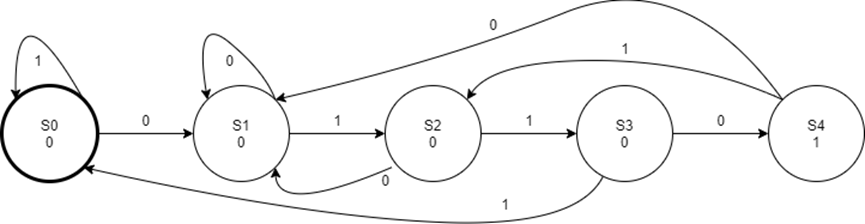
\includegraphics[width=0.8\textwidth]{assets/graph_fsm_1.png}
    \caption{检测序列 0110 的状态机 状态转移图}
\end{figure}

\subsection{检测序列 1011 的状态机}

状态转移图如图所示:

\begin{figure}[H]
    \centering
    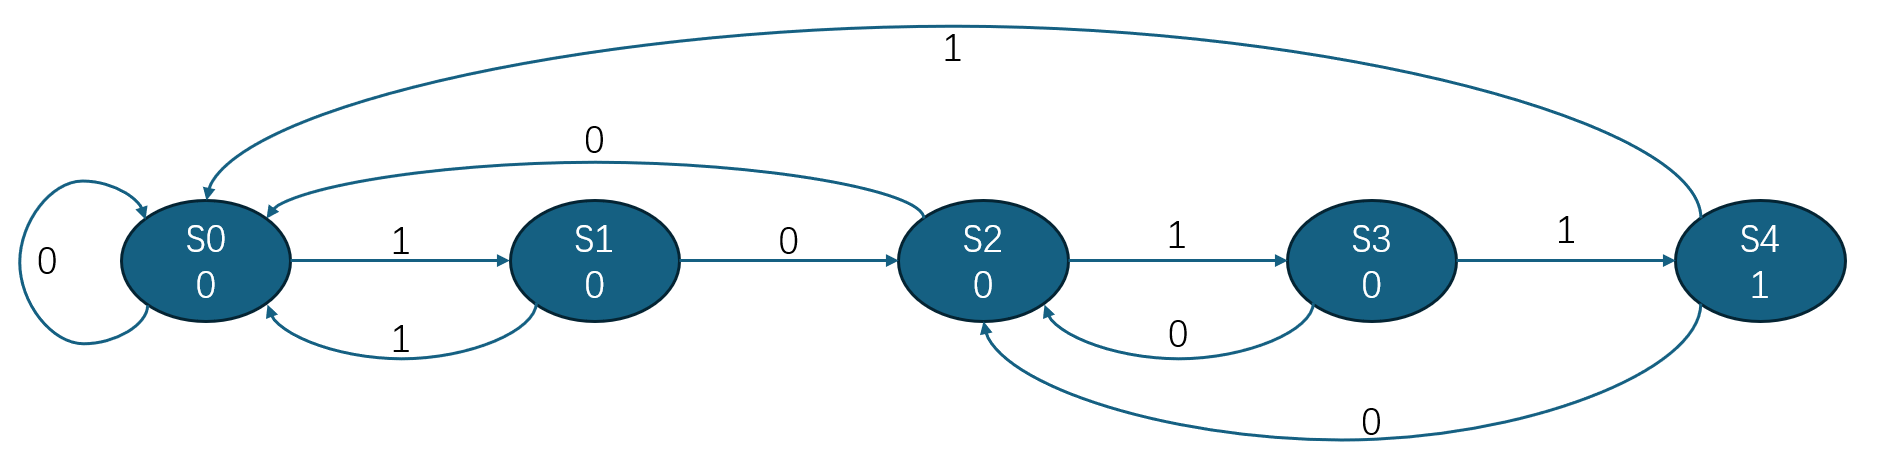
\includegraphics[width=0.8\textwidth]{assets/graph_fsm_2.png}
    \caption{检测序列 1011 的状态机 状态转移图}
\end{figure}

\subsection{序列信号发生器}

状态转移图如图所示:

\begin{figure}[H]
    \centering
    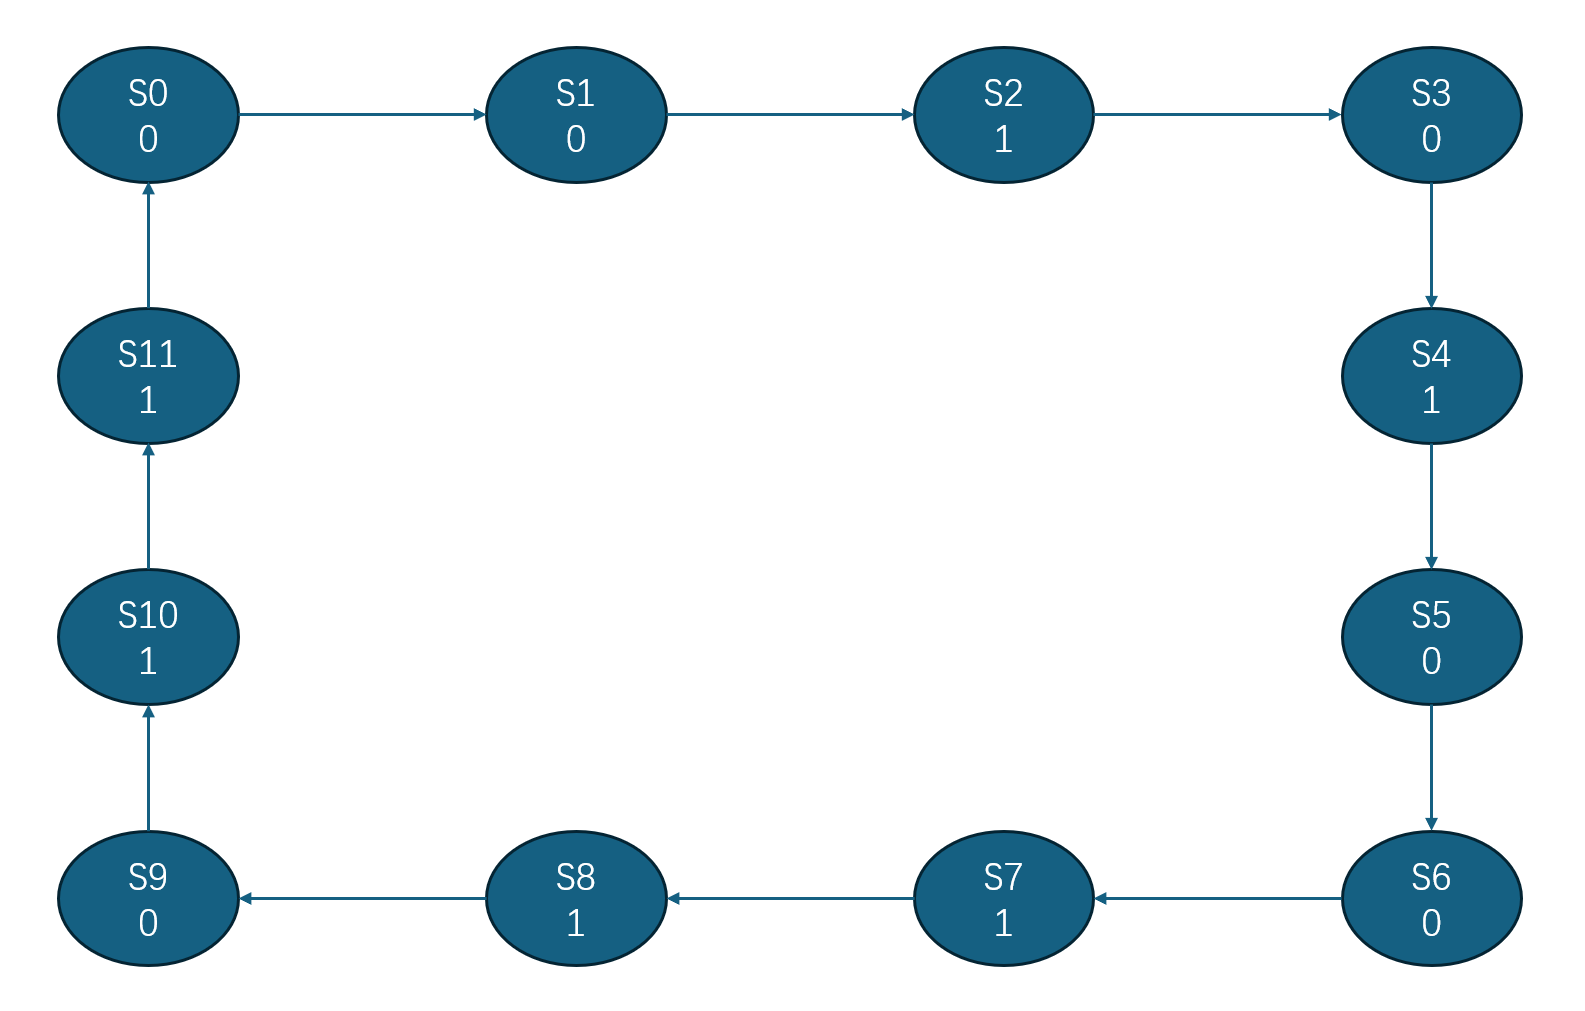
\includegraphics[width=0.8\textwidth]{assets/graph_ssg.png}
    \caption{序列信号发生器 状态转移图}
\end{figure}

\subsection{报纸售卖机}

报纸售卖机一共有 6 个状态: \(S0\) 为初始状态, \(S1\) 为已经投入 1 分钱的状态, \(S2\) 为已经投入 2 分钱的状态, \(S3\) 为已经投入 3 分钱的状态, \(S4\) 为已经投入 4 分钱的状态, \(S5\) 为已经投入不小于 5 分钱 (可以吐出报纸) 的状态. \(S5\) 输出 1, 剩余状态均输出 0. 状态转移图如图所示:

\begin{figure}[H]
    \centering
    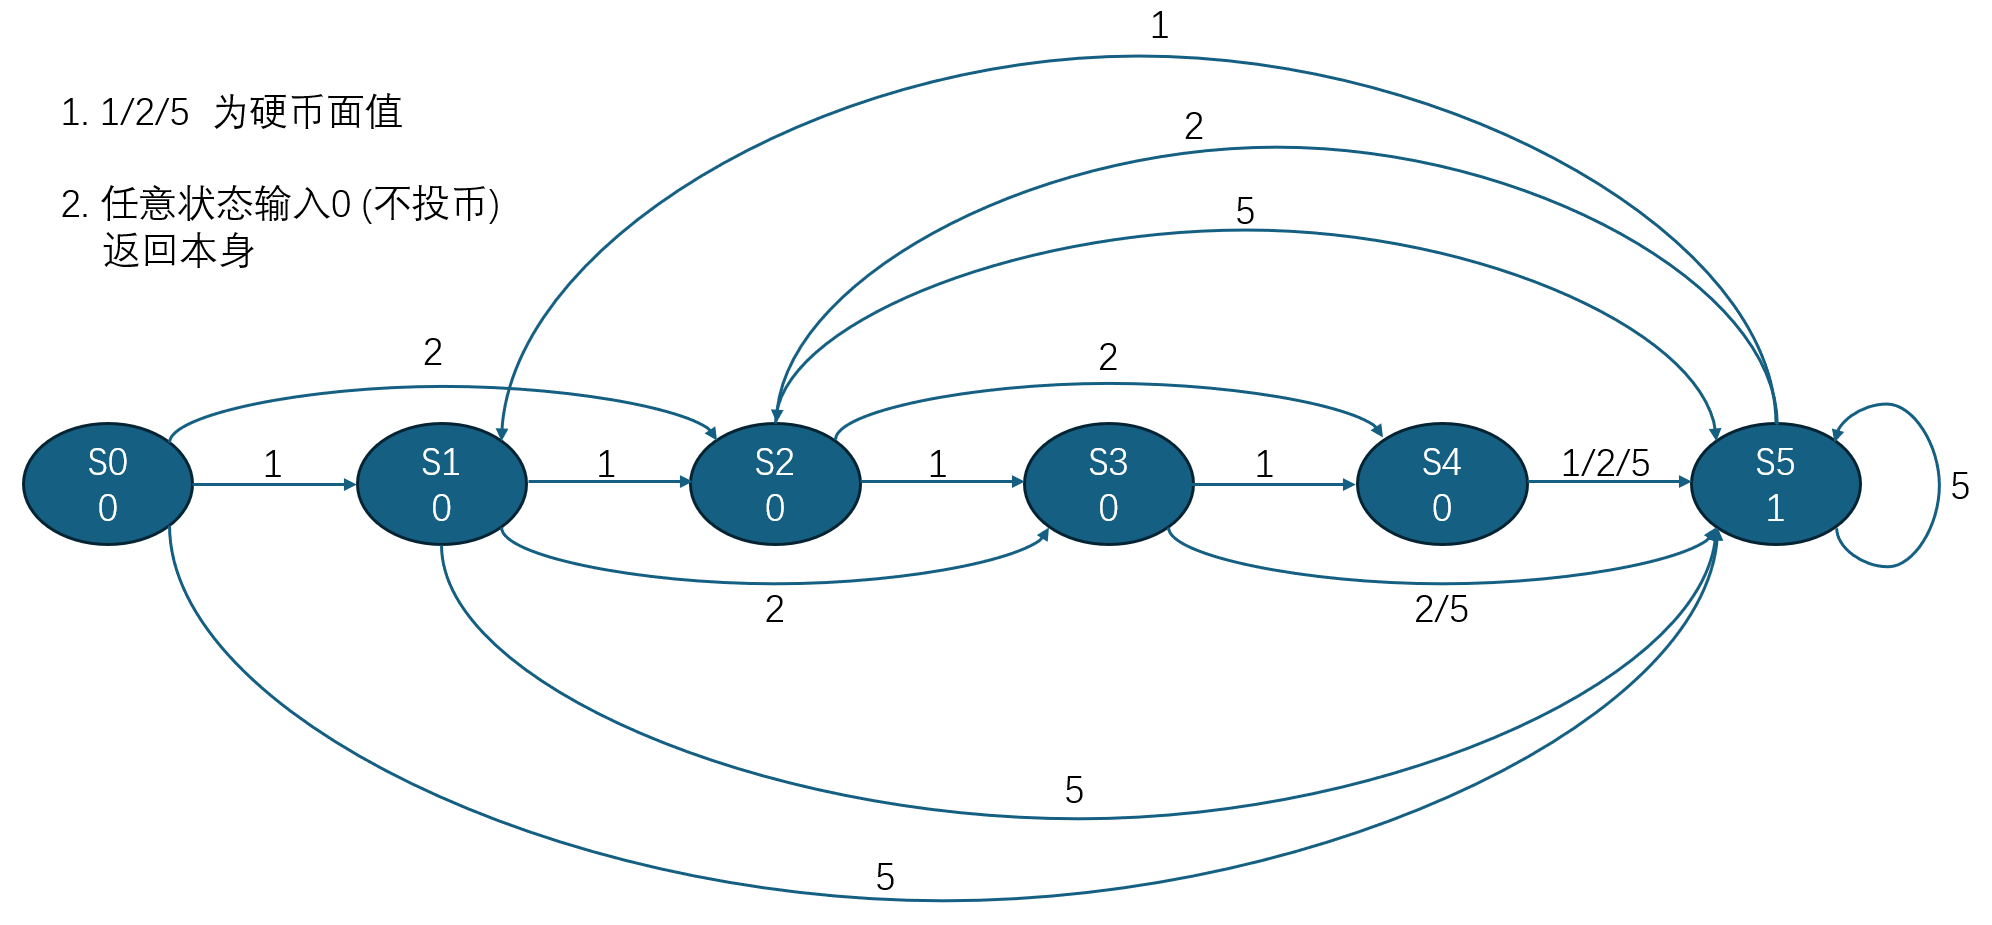
\includegraphics[width=0.9\textwidth]{assets/graph_ns.png}
    \caption{报纸售卖机 状态转移图}
\end{figure}

\section{接口定义}

\subsection{检测序列 0110 的状态机}

\begin{lstlisting}
    input clk,          // 时钟信号
    input rstn,         // 复位信号
    input in,           // 输入信号
    output reg out      // (寄存器) 输出信号
\end{lstlisting}

\subsection{检测序列 1011 的状态机}

\begin{lstlisting}
    input clk,           // 时钟信号
    input rstn,          // 复位信号
    input in,            // 输入信号
    output reg out       // (寄存器) 输出信号
\end{lstlisting}

\subsection{序列信号发生器}

\begin{lstlisting}  
    input clk,          // 时钟信号
    input rstn,         // 复位信号
    output reg out      // (寄存器) 输出信号
\end{lstlisting}

\subsection{报纸售卖机}

\begin{lstlisting}
    input clk,          // 时钟信号
    input rstn,         // 复位信号
    input [1:0] in,     // 输入信号         // in = 1 表示投入1分硬币
                                            // in = 2 表示投入2分硬币
                                            // in = 3 表示投入5分硬币
    output reg out      // (寄存器) 输出信号,   out = 1 表示机器吐出一份报纸
\end{lstlisting}


\section{调试过程及结果}

点击左侧 ``SIMULATION'' 下的 ``Run Simulation'', 以默认设置进行模拟调试. 调试结果分别如图所示:

\subsection{检测序列 0110 的状态机}

\begin{figure}[H]
    \centering
    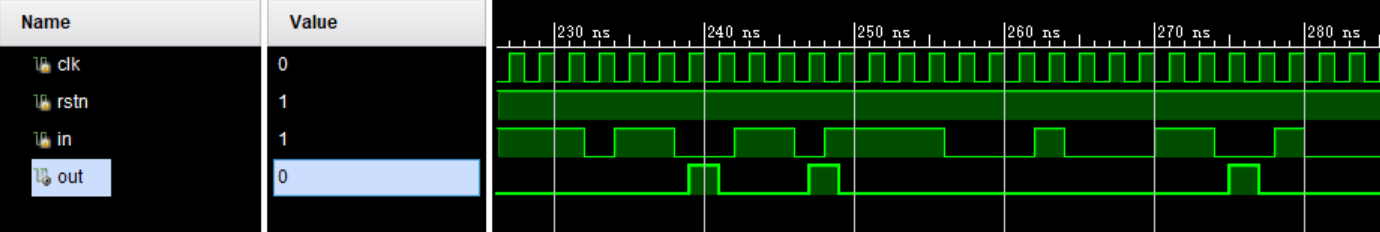
\includegraphics[width=0.98\textwidth]{assets/fsm_1.png}
    \caption{检测序列 0110 的状态机 模拟示意图}
\end{figure}

\subsection{检测序列 1011 的状态机}

\begin{figure}[H]
    \centering
    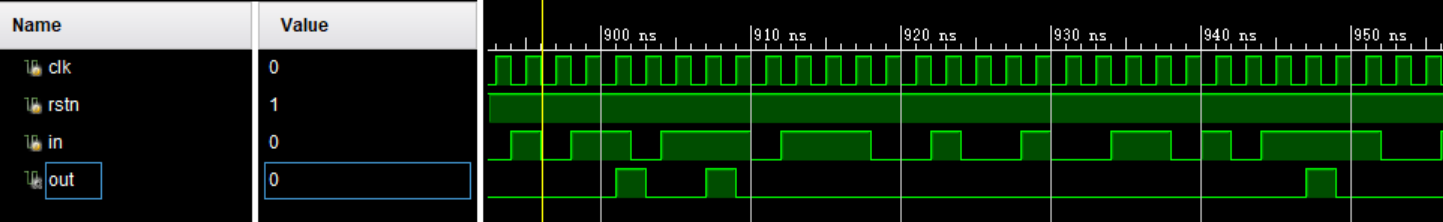
\includegraphics[width=0.98\textwidth]{assets/fsm_2.png}
    \caption{检测序列 0110 的状态机 模拟示意图}
\end{figure}

\subsection{序列信号发生器}

\begin{figure}[H]
    \centering
    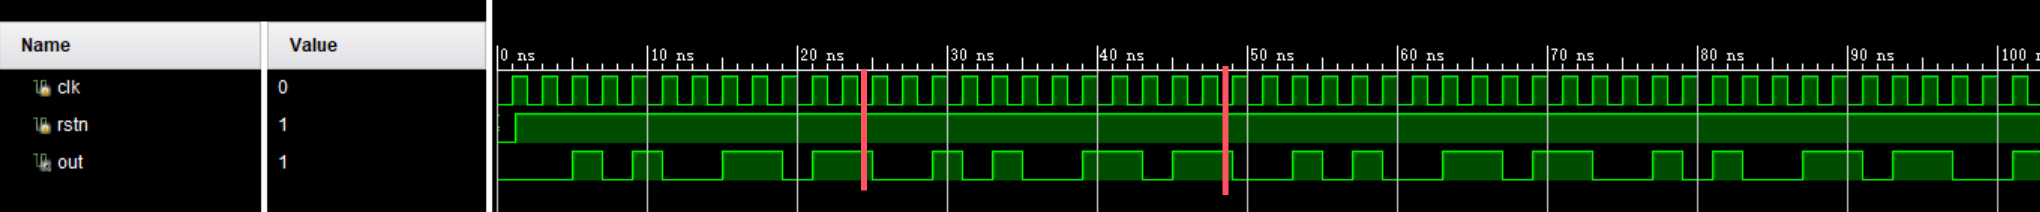
\includegraphics[width=0.98\textwidth]{assets/sequence_signal_generator.png}
    \caption{序列信号发生器 模拟示意图}
\end{figure}

\subsection{报纸售卖机}

\begin{figure}[H]
    \centering
    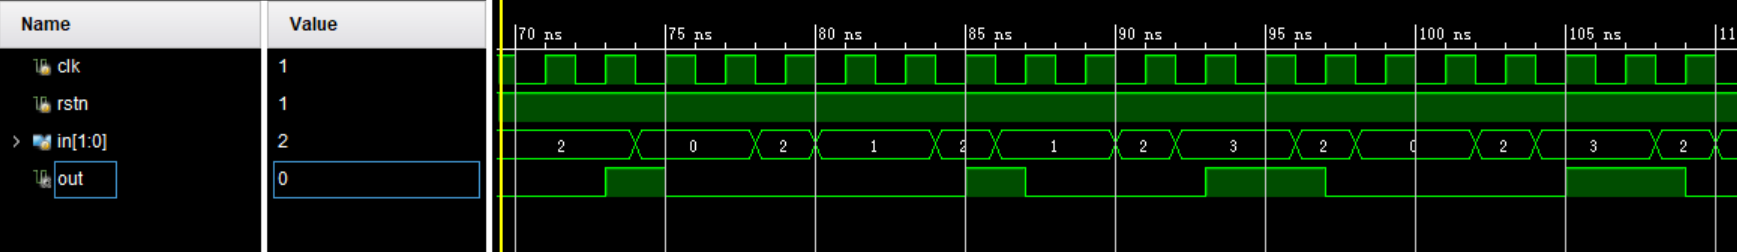
\includegraphics[width=0.98\textwidth]{assets/newspaper_seller.png}
    \caption{报纸售卖机 模拟示意图}
\end{figure}

\section{实验总结}

通过本次实验, 我了解并实践了状态机设计的方法, 学习了时序电路和非阻塞赋值的应用, 对有限状态机的结构有了更深刻的认识.

\section{源代码}

\subsection{检测序列 0110 的状态机}

File: fsm\_1.v
\begin{lstlisting}
    `timescale 1ns / 1ps

    module fsm_1(
        input clk,
        input rstn,
        input in,
        output reg out
        );
        
        localparam [2:0] S0 = 3'b0;
        localparam [2:0] S1 = 3'b1;
        localparam [2:0] S2 = 3'b10;
        localparam [2:0] S3 = 3'b11;
        localparam [2:0] S4 = 3'b100;
        
        
        reg [2:0] state = 3'b0;
        reg [2:0] next_state;
        
        always @(posedge clk or negedge rstn) begin
            if (!rstn) begin
                state <= S0;
            end
            else begin
                state <= next_state;
            end
        end
        
        always @(in or state) begin
            case(state)
            S0: next_state = in ? S0 : S1;
            S1: next_state = in ? S2 : S1;
            S2: next_state = in ? S3 : S1;
            S3: next_state = in ? S0 : S4;
            S4: next_state = in ? S2 : S1;
            default: next_state = S0;
            endcase
        end

        always @(state) begin
            case(state)
            S0: out = 1'b0;
            S1: out = 1'b0;
            S2: out = 1'b0;
            S3: out = 1'b0;
            S4: out = 1'b1;
            default: out = 1'bx;
            endcase
        end
    endmodule
\end{lstlisting}

File: test\_fsm\_1.v
\begin{lstlisting}
    `timescale 1ns / 1ps

    module test_fsm();

        reg clk;
        reg rstn;
        reg in;
        wire out;

        fsm_1 inst_fsm_1(
            .clk(clk),
            .rstn(rstn),
            .in(in),
            .out(out)
        );

        initial begin
            clk = 0;
            rstn = 1;
            #0.1 rstn = 0;
            #1.1 rstn = 1;
        end

        initial begin
            in = 0;
            #4 in = 1;
            #4 in = 0;
        end

        always begin
            #1 clk = ~clk;
        end

        always begin
            #2 in = $random() % 2;
        end
    endmodule

\end{lstlisting}

\subsection{检测序列 1011 的状态机}

File: fsm\_2.v
\begin{lstlisting}
    `timescale 1ns / 1ps

    module fsm_2(
        input clk,
        input rstn,
        input in,
        output reg out
        );
         
        localparam [2:0] S0 = 3'b0;
        localparam [2:0] S1 = 3'b1;
        localparam [2:0] S2 = 3'b10;
        localparam [2:0] S3 = 3'b11;
        localparam [2:0] S4 = 3'b100;
        
        
        reg [2:0] state = 3'b0;
        reg [2:0] next_state;
        
        always @(posedge clk or negedge rstn) begin
            if (!rstn) begin
                state <= S0;
            end
            else begin
                state <= next_state;
            end
        end
        
        always @(in or state) begin
            case(state)
            S0: next_state = in ? S1 : S0;
            S1: next_state = in ? S0 : S2;
            S2: next_state = in ? S3 : S0;
            S3: next_state = in ? S4 : S2;
            S4: next_state = in ? S0 : S2;
            default: next_state = S0;
            endcase
        end
    
        always @(state) begin
            case(state)
            S0: out = 1'b0;
            S1: out = 1'b0;
            S2: out = 1'b0;
            S3: out = 1'b0;
            S4: out = 1'b1;
            default: out = 1'bx;
            endcase
        end
    endmodule
    
\end{lstlisting}

File: test\_fsm\_2.v
\begin{lstlisting}
    `timescale 1ns / 1ps


    module test_fsm();

        reg clk;
        reg rstn;
        reg in;
        wire out;

        fsm_2 inst_fsm_2(
            .clk(clk),
            .rstn(rstn),
            .in(in),
            .out(out)
        );

        initial begin
            clk = 0;
            rstn = 1;
            #0.1 rstn = 0;
            #1.1 rstn = 1;
        end

        initial begin
            in = 0;
            #4 in = 1;
            #4 in = 0;
        end

        always begin
            #1 clk = ~clk;
        end

        always begin
            #2 in = $random() % 2;
        end
    endmodule

\end{lstlisting}

\subsection{序列信号发生器}

File: sequence\_signal\_generator.v
\begin{lstlisting}
    `timescale 1ns / 1ps

    module sequence_signal_generator(
        input clk,
        input rstn,
        output reg out
        );
         
        localparam [3:0] S0 = 4'b0000;
        localparam [3:0] S1 = 4'b0001;
        localparam [3:0] S2 = 4'b0010;
        localparam [3:0] S3 = 4'b0011;
        localparam [3:0] S4 = 4'b0100;
        localparam [3:0] S5 = 4'b0101;
        localparam [3:0] S6 = 4'b0110;
        localparam [3:0] S7 = 4'b0111;
        localparam [3:0] S8 = 4'b1000;
        localparam [3:0] S9 = 4'b1001;
        localparam [3:0] S10 = 4'b1010;
        localparam [3:0] S11 = 4'b1011;
    
        
        
        reg [3:0] state = S0;
        reg [3:0] next_state;
        
        always @(posedge clk or negedge rstn) begin
            if (!rstn) begin
                state <= S0;
            end
            else begin
                state <= next_state;
            end
        end
        
        always @(state) begin
            case(state)
            S0: next_state = S1;
            S1: next_state = S2;
            S2: next_state = S3;
            S3: next_state = S4;
            S4: next_state = S5;
            S5: next_state = S6;
            S6: next_state = S7;
            S7: next_state = S8;
            S8: next_state = S9;
            S9: next_state = S10;
            S10: next_state = S11;
            S11: next_state = S0;
            default: next_state = S0;
            endcase
        end
    
        always @(state) begin
            case(state)
            S0: out = 1'b0;
            S1: out = 1'b0;
            S3: out = 1'b0;
            S5: out = 1'b0;
            S6: out = 1'b0;
            S9: out = 1'b0;
            S2: out = 1'b1;
            S4: out = 1'b1;
            S7: out = 1'b1;
            S8: out = 1'b1;
            S10: out = 1'b1;
            S11: out = 1'b1;
            default: out = 1'bx;
            endcase
        end
    endmodule    
\end{lstlisting}

File: test\_sequence\_signal\_generator.v
\begin{lstlisting}
    `timescale 1ns / 1ps


    module test_sequence_signal_generator();
    
        reg clk;
        reg rstn;
        wire out;
    
        sequence_signal_generator inst_sequence_signal_generator(
            .clk(clk),
            .rstn(rstn),
            .out(out)
        );
    
        initial begin
            clk = 0;
            rstn = 1;
            #0.1 rstn = 0;
            #1.1 rstn = 1;
        end
    
        always begin
            #1 clk = ~clk;
        end
    endmodule    
\end{lstlisting}

\subsection{报纸售卖机}

File: newspaper\_seller.v
\begin{lstlisting}
    `timescale 1ns / 1ps

    module newspaper_seller(
        input clk,
        input rstn,
        input [1:0] in,
        output reg out
        );
    
        // in = 1 表示投入1分硬币
        // in = 2 表示投入2分硬币
        // in = 3 表示投入5分硬币
         
        localparam [2:0] S0 = 3'b000;
        localparam [2:0] S1 = 3'b001;
        localparam [2:0] S2 = 3'b010;
        localparam [2:0] S3 = 3'b011;
        localparam [2:0] S4 = 3'b100;
        localparam [2:0] S5 = 3'b101;
    
        reg [3:0] state = S0;
        reg [3:0] next_state;
        
        always @(posedge clk or negedge rstn) begin
            if (!rstn) begin
                state <= S0;
            end
            else begin
                state <= next_state;
            end
        end
        
        always @(in or state) begin
            case(state)
            S0: begin
                if (in == 2'b01)
                    next_state = S1;
                else if (in == 2'b10)
                    next_state = S2;
                else if (in == 2'b11)
                    next_state = S5;
                else
                    next_state = S0;
            end
            S1: begin
                if (in == 2'b01)
                    next_state = S2;
                else if (in == 2'b10)
                    next_state = S3;
                else if (in == 2'b11)
                    next_state = S5;
                else
                    next_state = S1;
            end
            S2: begin
                if (in == 2'b01)
                    next_state = S3;
                else if (in == 2'b10)
                    next_state = S4;
                else if (in == 2'b11)
                    next_state = S5;
                else
                    next_state = S2;
            end
            S3: begin
                if (in == 2'b01)
                    next_state = S4;
                else if (in == 2'b10)
                    next_state = S5;
                else if (in == 2'b11)
                    next_state = S5;
                else
                    next_state = S3;
            end
            S4: begin
                if (in == 2'b01)
                    next_state = S5;
                else if (in == 2'b10)
                    next_state = S5;
                else if (in == 2'b11)
                    next_state = S5;
                else
                    next_state = S4;
            end
            S5: begin
                if (in == 2'b01)
                    next_state = S1;
                else if (in == 2'b10)
                    next_state = S2;
                else if (in == 2'b11)
                    next_state = S5;
                else
                    next_state = S0;
            end
    
            default: next_state = S0;
            endcase
        end
    
        always @(state) begin
            case(state)
            S5: out = 1'b1;
            S0: out = 1'b0;
            S1: out = 1'b0;
            S2: out = 1'b0;
            S3: out = 1'b0;
            S4: out = 1'b0;
            default: out = 1'bx;
            endcase
        end
    endmodule    
\end{lstlisting}

File: test\_newspaper\_seller.v
\begin{lstlisting}
    `timescale 1ns / 1ps


    module test_newspaper_seller();
        reg clk;
        reg rstn;
        reg [1:0] in;
        wire out;
    
        newspaper_seller inst_newspaper_seller(
            .clk(clk),
            .rstn(rstn),
            .in(in),
            .out(out)
        );
    
        initial begin
            clk = 0;
            rstn = 1;
            #0.1 rstn = 0;
            #1.1 rstn = 1;
        end
    
        initial begin
            in = 0;
        end
    
        always begin
            #1 clk = ~clk;
        end
    
        always begin
            #2 in = $random() % 3;
            #4 in = 2'b10;
        end
    endmodule    
\end{lstlisting}

\end{document}